\section{Anexos}

\begin{figure}[H]
  \centering
  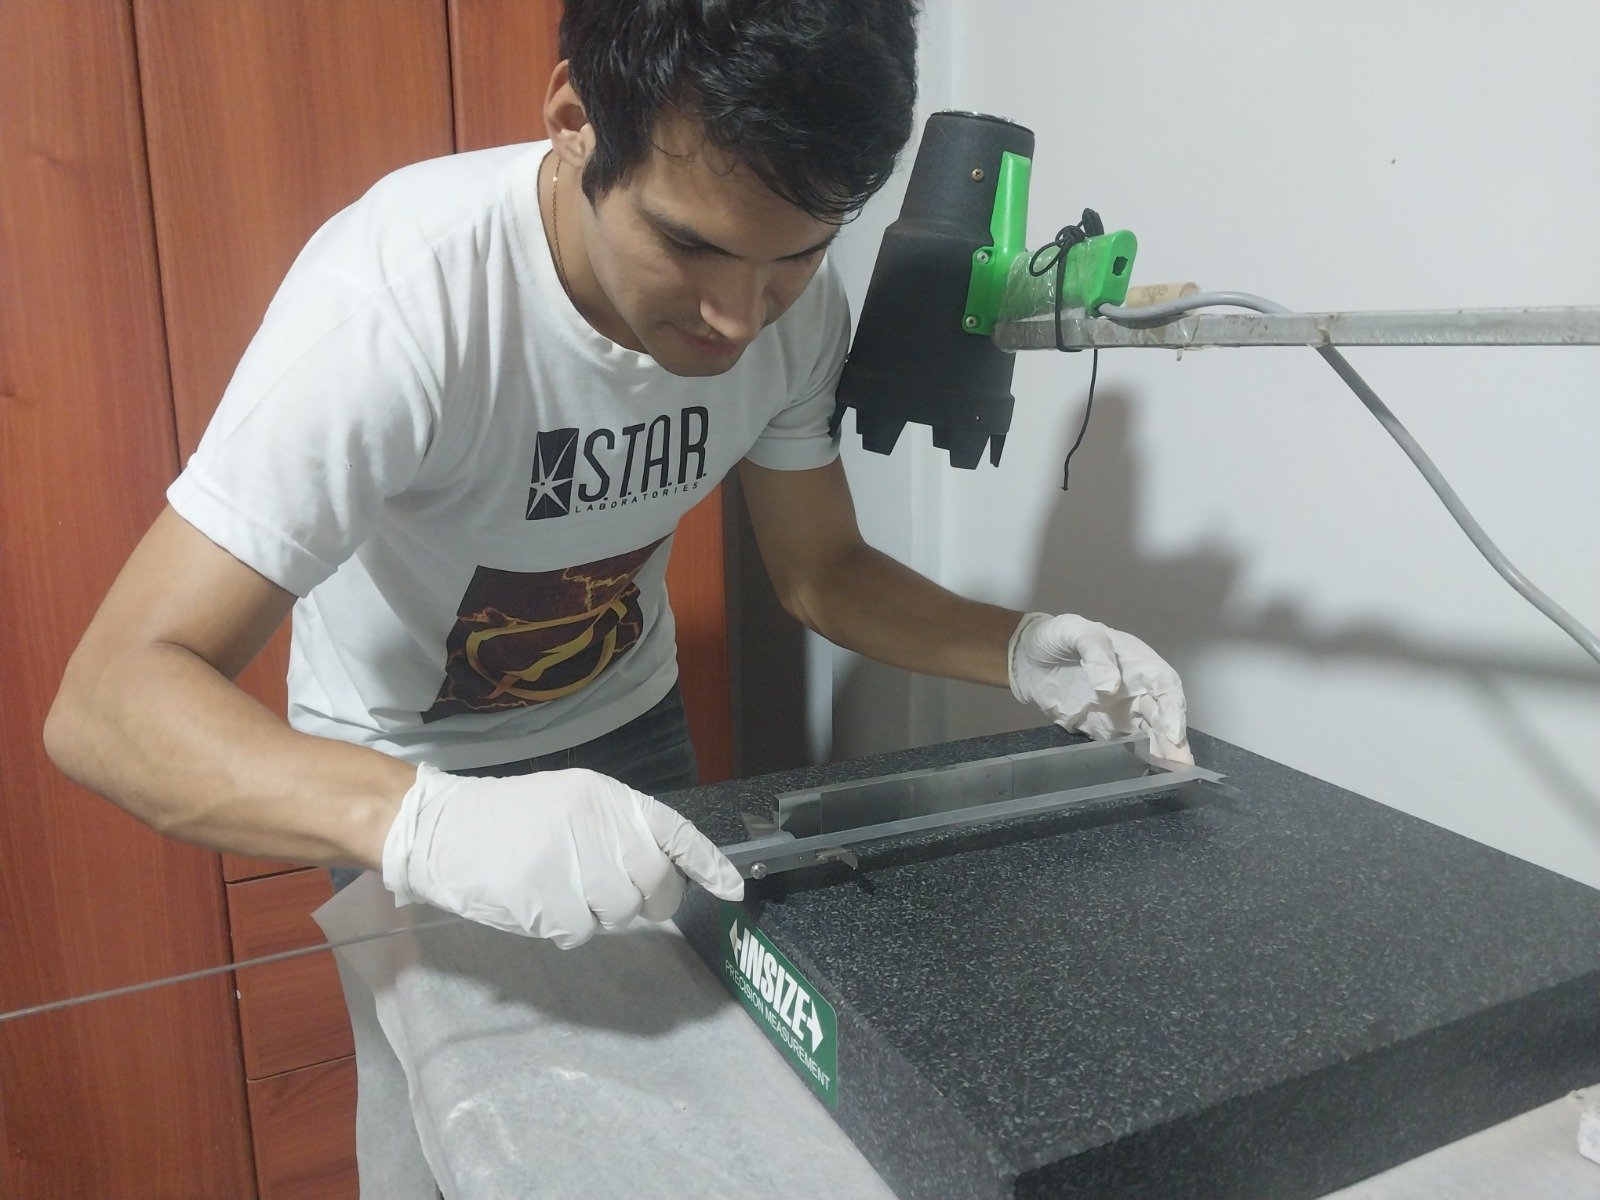
\includegraphics[width=0.5\textwidth]{img/Meausre_pie_de_rey.jpeg}
  \caption{Pie de rey Mitutoyo 530-115 durante la medición sobre la mesa de
  granito.}
  \label{fig:anexo-pie-de-rey}
\end{figure}

\begin{figure}[H]
  \centering
  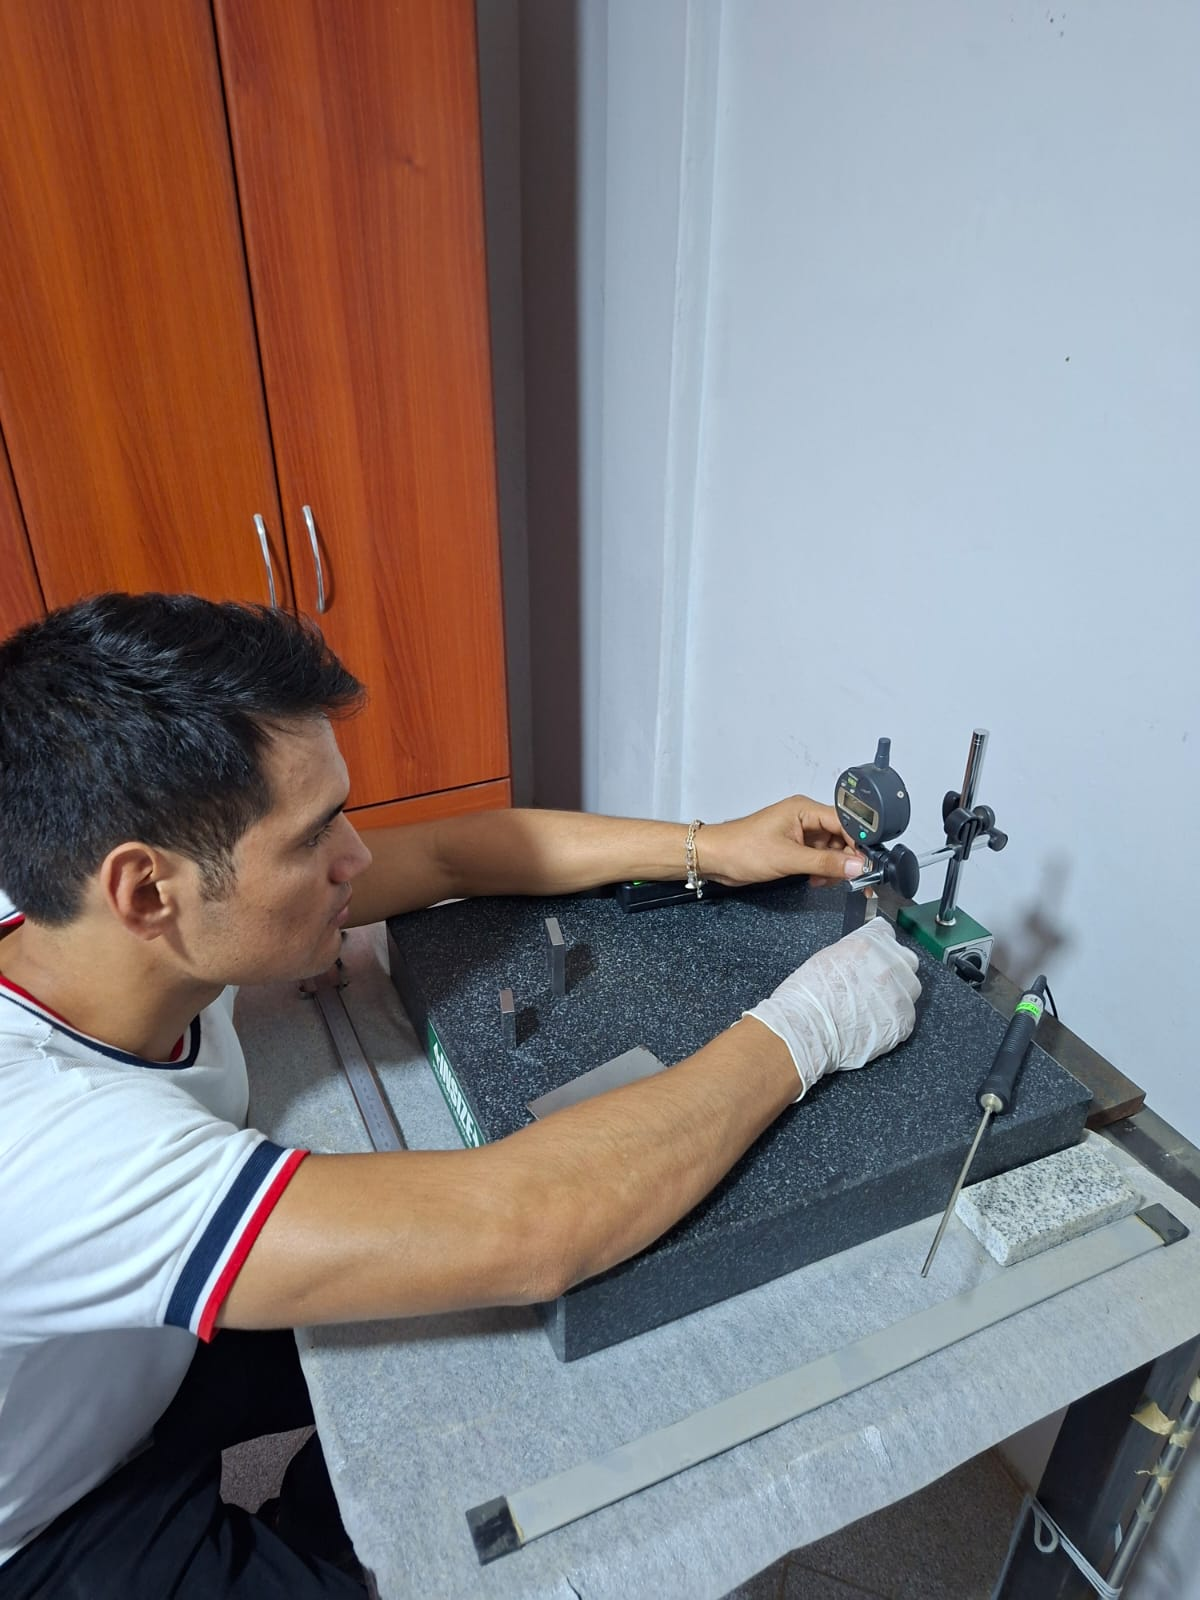
\includegraphics[width=0.42\textwidth]{img/measure_comparator_clock.jpeg}
  \caption{Comparador digital Mitutoyo ID-S1012M sobre la mesa de granito, con
  bloques patrón.}
  \label{fig:anexo-comparador}
\end{figure}

\begin{figure}[H]
  \centering
  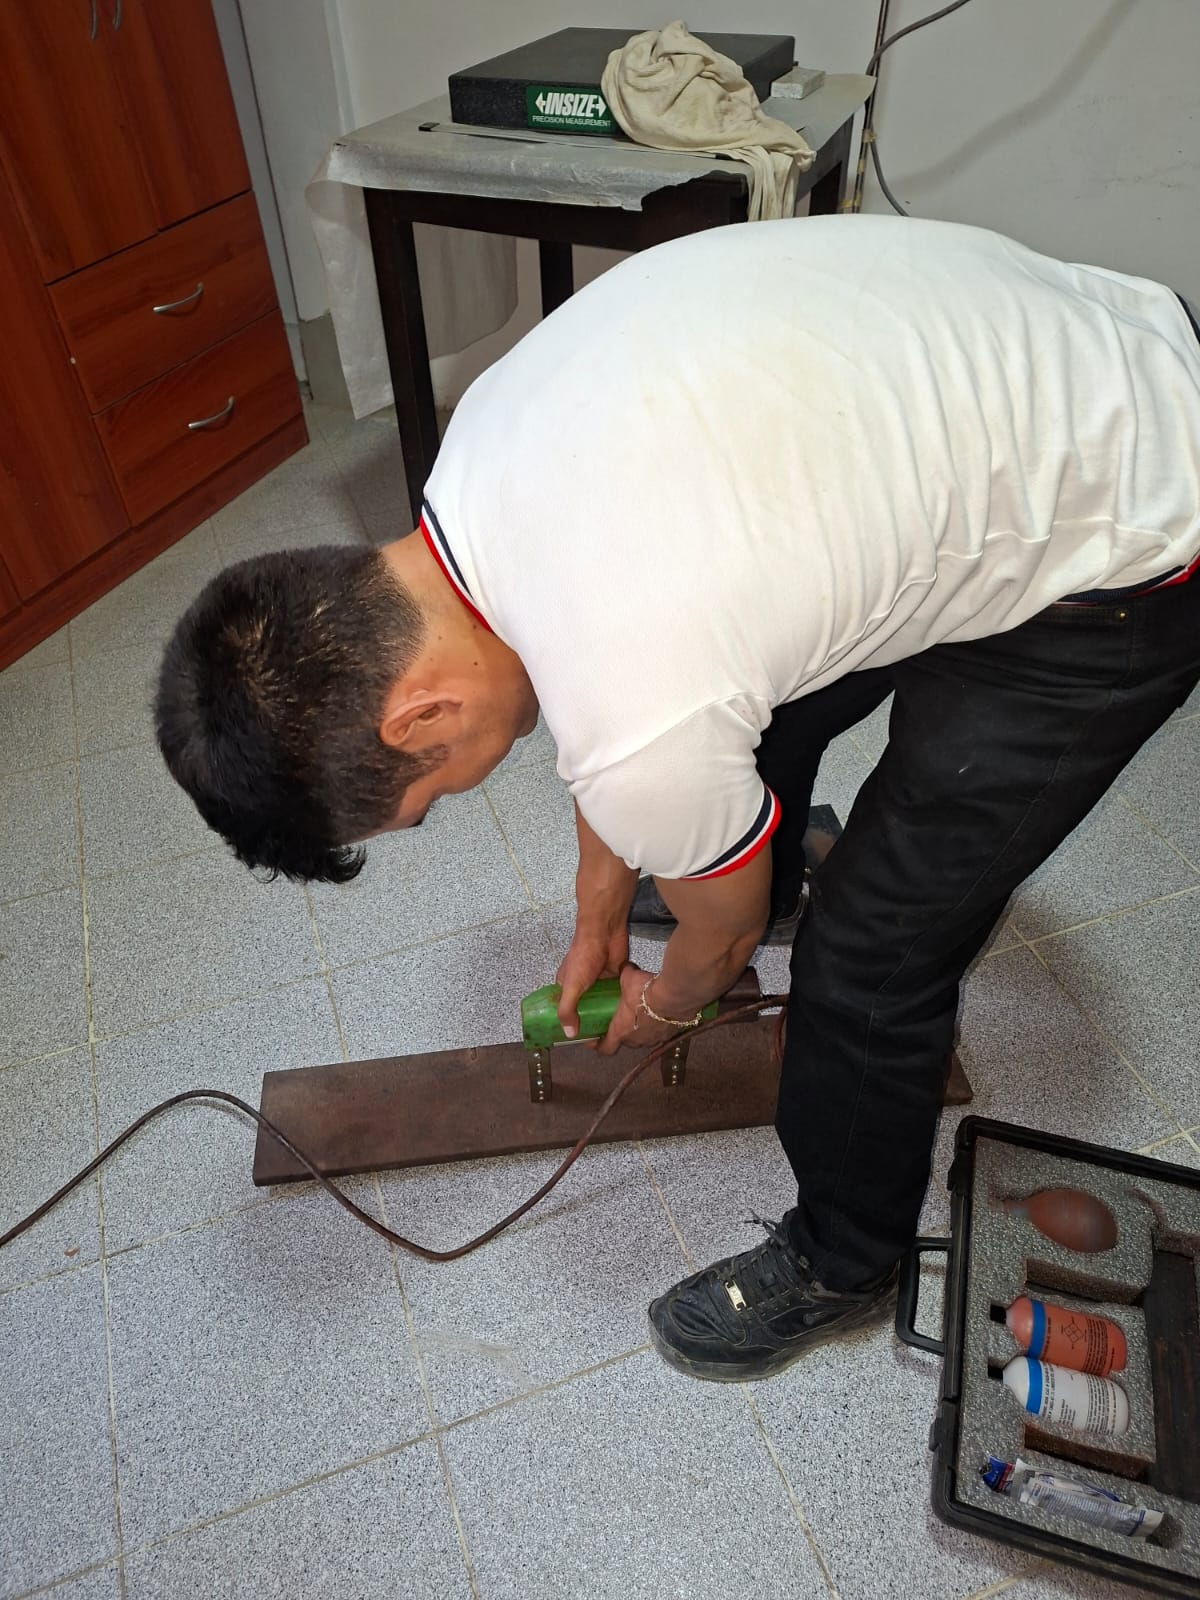
\includegraphics[width=0.42\textwidth]{img/magnetic_yugo_measure.jpeg}
  \caption{Yugo Magnaflux Y-7 sobre una placa de acero durante la inspección.}
  \label{fig:anexo-yugo}
\end{figure}

\begin{figure}[H]
  \centering
  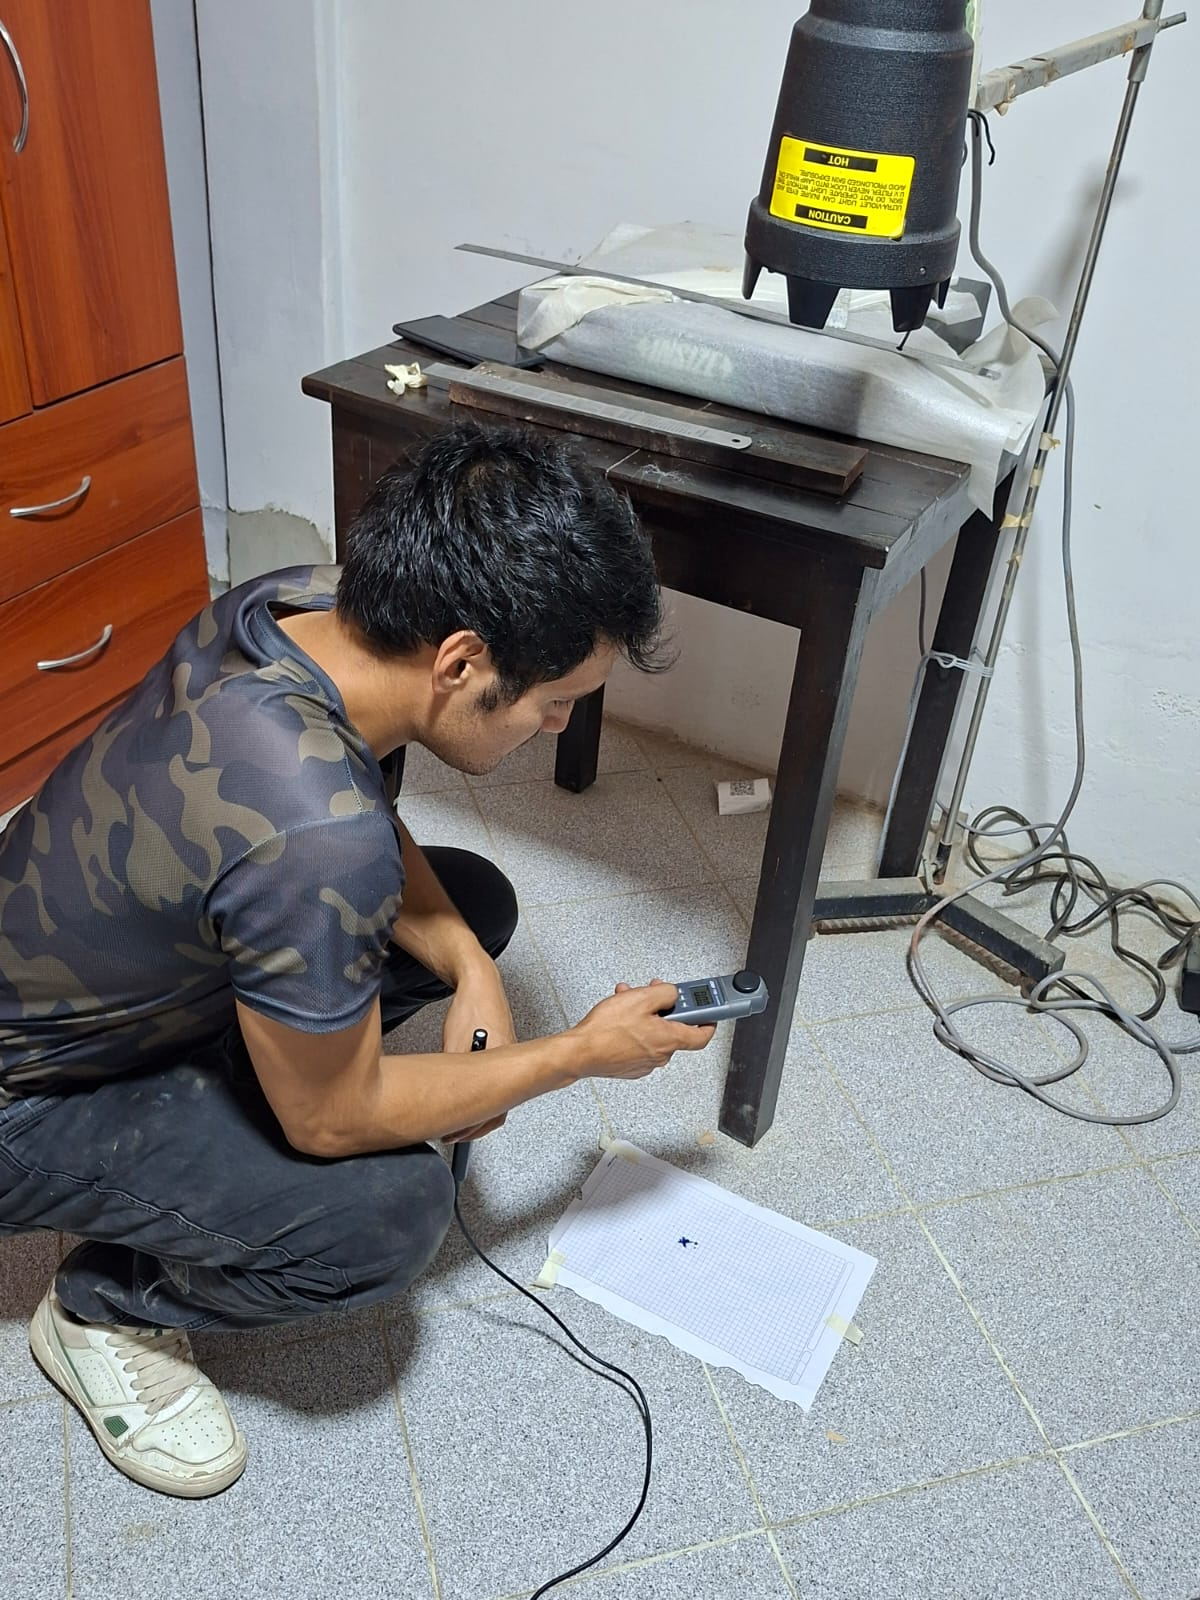
\includegraphics[width=0.42\textwidth]{img/measure_black_light_lampera.jpeg}
  \caption{Medición de intensidad de lámpara UV.}
  \label{fig:anexo-uv-lampara}
\end{figure}

\begin{figure}[H]
  \centering
  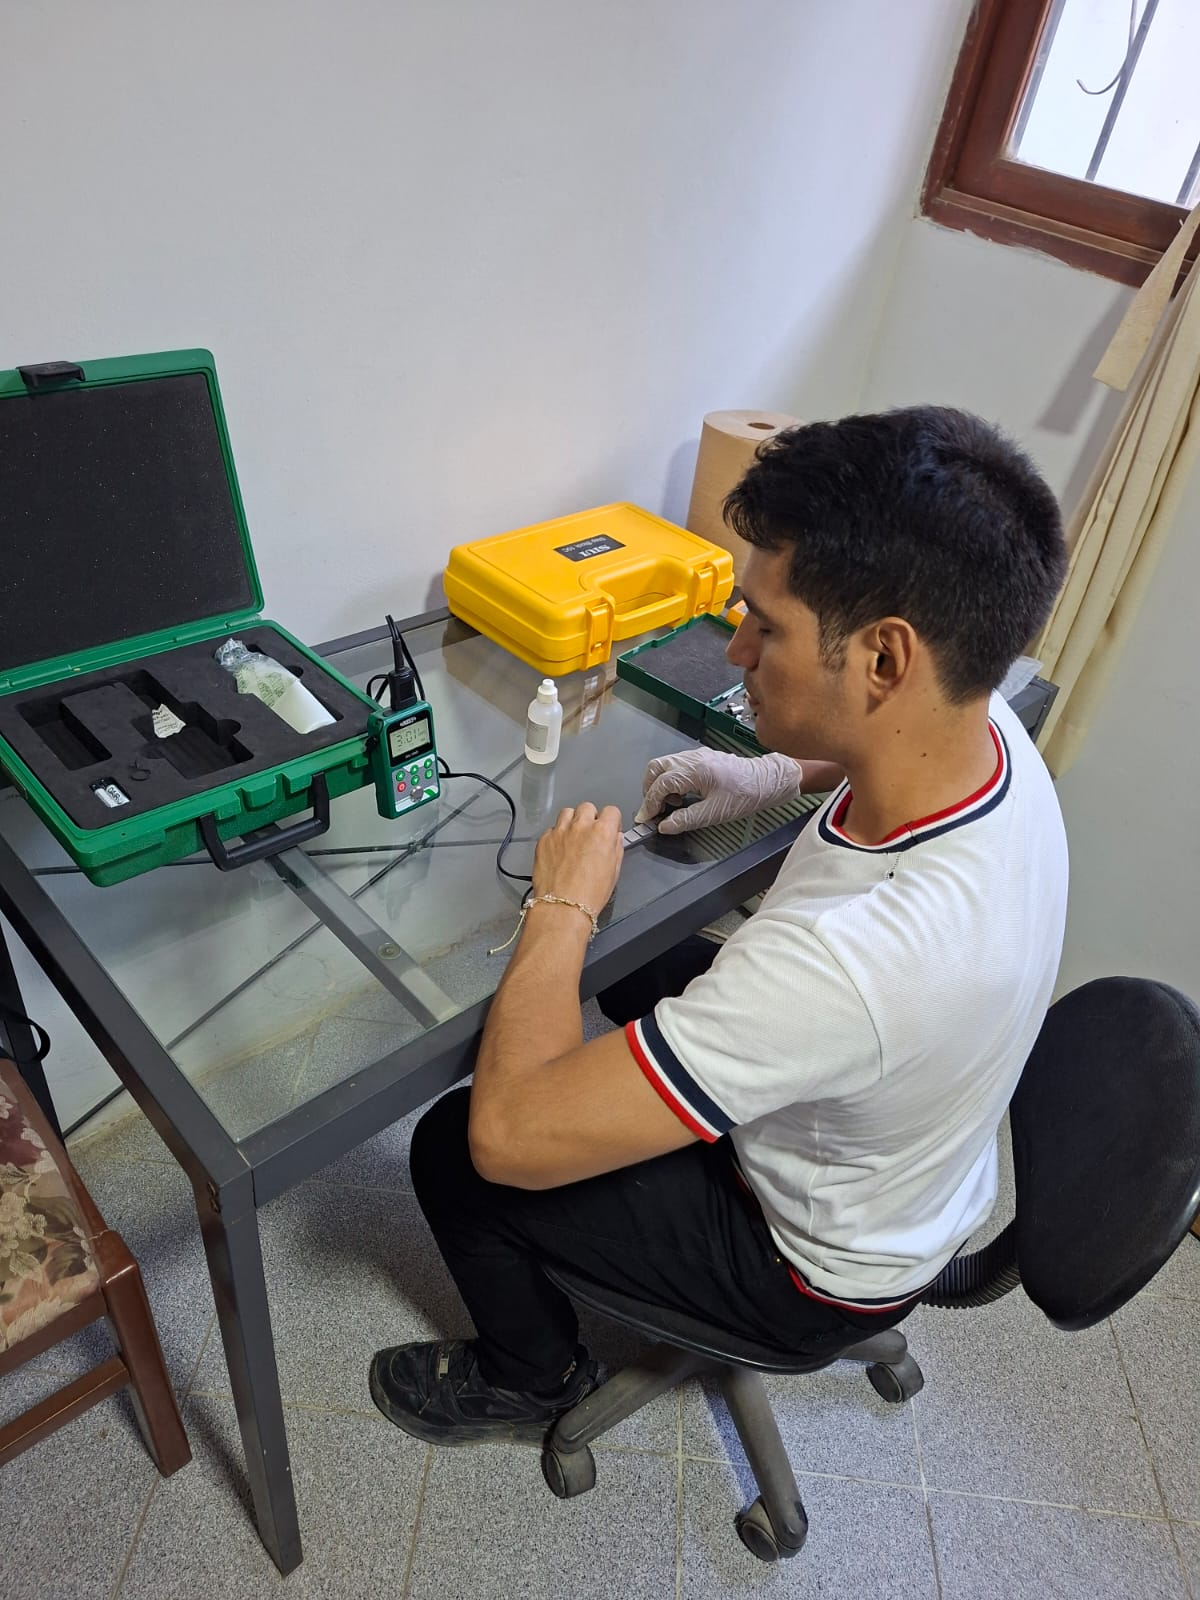
\includegraphics[width=0.42\textwidth]{img/measure_ultrasound.jpeg}
  \caption{Medición de espesores con el ISU-100D sobre el bloque escalonado.}
  \label{fig:anexo-ut-medicion}
\end{figure}

\begin{figure}[H]
  \centering
  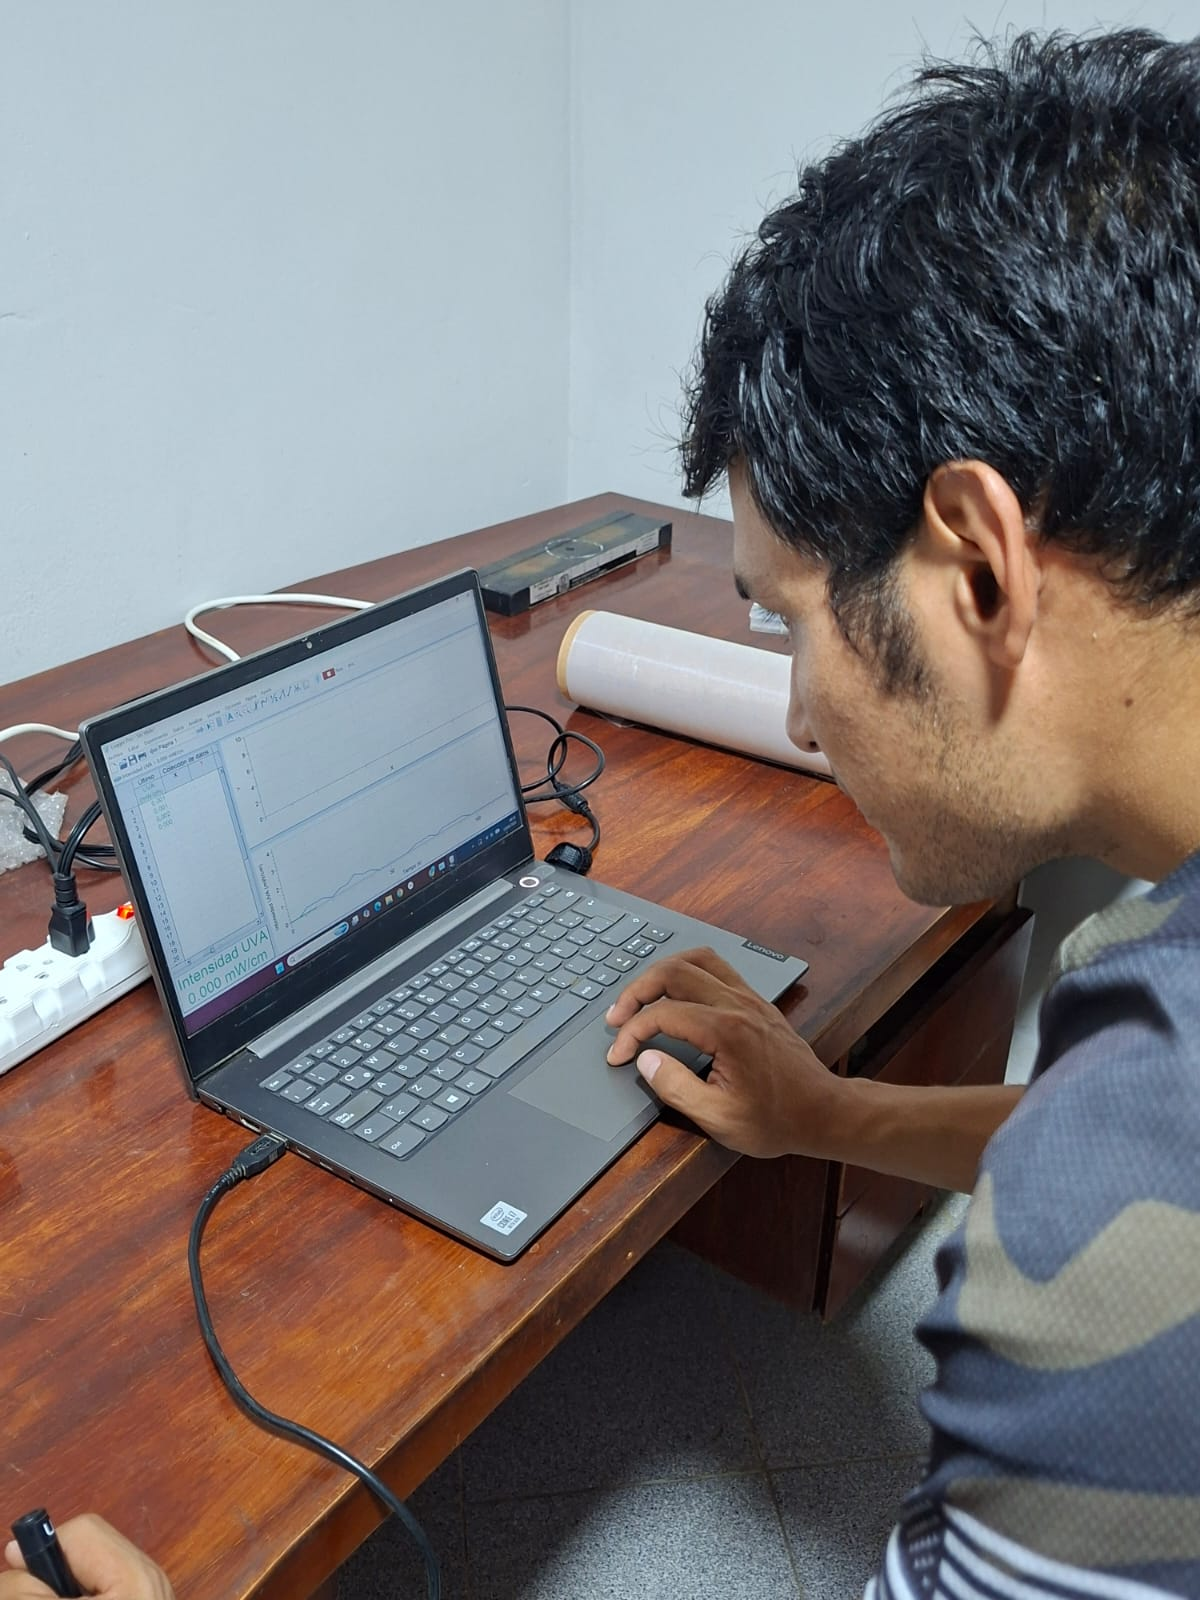
\includegraphics[width=0.42\textwidth]{img/view_measure_radiation_black_light_lampera.jpeg}
  \caption{Lectura de intensidad UV-A en el registrador.}
  \label{fig:anexo-uv-intensidad}
\end{figure}

\todo{Incorporar los certificados de calibración y el código de los notebooks.}
